% Created by tikzDevice version 0.10.1 on 2016-06-30 12:40:44
% !TEX encoding = UTF-8 Unicode
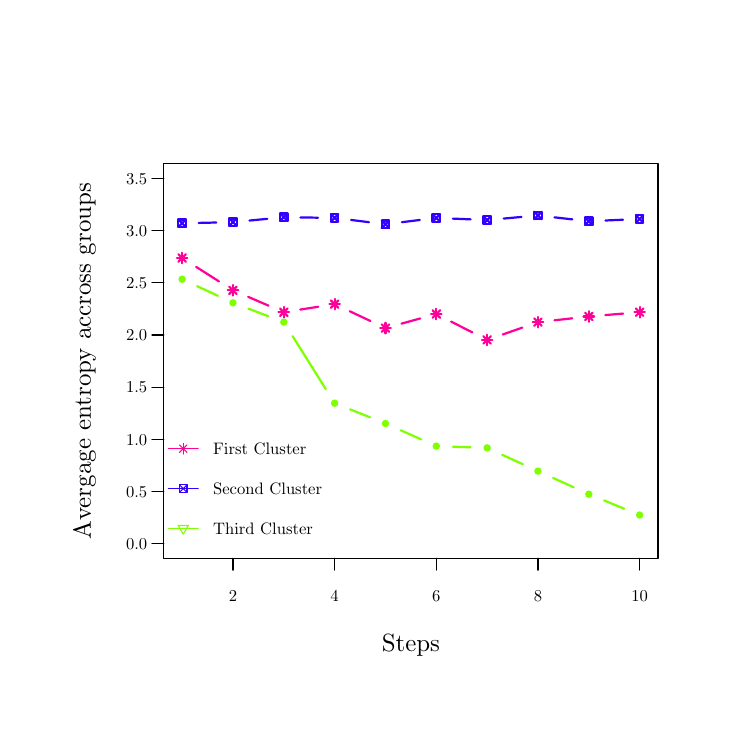
\begin{tikzpicture}[x=1pt,y=1pt]
\definecolor{fillColor}{RGB}{255,255,255}
\path[use as bounding box,fill=fillColor,fill opacity=0.00] (0,0) rectangle (252.94,252.94);
\begin{scope}
\path[clip] ( 49.20, 61.20) rectangle (227.75,203.75);
\definecolor{drawColor}{RGB}{255,0,153}

\path[draw=drawColor,line width= 0.8pt,line join=round,line cap=round] ( 60.88,166.49) -- ( 69.12,161.26);

\path[draw=drawColor,line width= 0.8pt,line join=round,line cap=round] ( 79.69,155.66) -- ( 87.04,152.49);

\path[draw=drawColor,line width= 0.8pt,line join=round,line cap=round] ( 98.48,151.06) -- (104.99,152.09);

\path[draw=drawColor,line width= 0.8pt,line join=round,line cap=round] (116.35,150.48) -- (123.86,146.94);

\path[draw=drawColor,line width= 0.8pt,line join=round,line cap=round] (135.07,145.98) -- (141.87,147.87);

\path[draw=drawColor,line width= 0.8pt,line join=round,line cap=round] (153.00,146.74) -- (160.68,142.82);

\path[draw=drawColor,line width= 0.8pt,line join=round,line cap=round] (171.69,142.08) -- (178.73,144.55);

\path[draw=drawColor,line width= 0.8pt,line join=round,line cap=round] (190.36,147.20) -- (196.80,147.92);

\path[draw=drawColor,line width= 0.8pt,line join=round,line cap=round] (208.74,149.09) -- (215.15,149.62);

\path[draw=drawColor,line width= 0.8pt,line join=round,line cap=round] ( 54.46,168.36) -- ( 57.16,171.06);

\path[draw=drawColor,line width= 0.8pt,line join=round,line cap=round] ( 54.46,171.06) -- ( 57.16,168.36);

\path[draw=drawColor,line width= 0.8pt,line join=round,line cap=round] ( 53.90,169.71) -- ( 57.72,169.71);

\path[draw=drawColor,line width= 0.8pt,line join=round,line cap=round] ( 55.81,167.80) -- ( 55.81,171.62);

\path[draw=drawColor,line width= 0.8pt,line join=round,line cap=round] ( 72.83,156.69) -- ( 75.53,159.39);

\path[draw=drawColor,line width= 0.8pt,line join=round,line cap=round] ( 72.83,159.39) -- ( 75.53,156.69);

\path[draw=drawColor,line width= 0.8pt,line join=round,line cap=round] ( 72.27,158.04) -- ( 76.09,158.04);

\path[draw=drawColor,line width= 0.8pt,line join=round,line cap=round] ( 74.18,156.13) -- ( 74.18,159.95);

\path[draw=drawColor,line width= 0.8pt,line join=round,line cap=round] ( 91.20,148.76) -- ( 93.90,151.46);

\path[draw=drawColor,line width= 0.8pt,line join=round,line cap=round] ( 91.20,151.46) -- ( 93.90,148.76);

\path[draw=drawColor,line width= 0.8pt,line join=round,line cap=round] ( 90.64,150.11) -- ( 94.46,150.11);

\path[draw=drawColor,line width= 0.8pt,line join=round,line cap=round] ( 92.55,148.20) -- ( 92.55,152.02);

\path[draw=drawColor,line width= 0.8pt,line join=round,line cap=round] (109.57,151.69) -- (112.27,154.39);

\path[draw=drawColor,line width= 0.8pt,line join=round,line cap=round] (109.57,154.39) -- (112.27,151.69);

\path[draw=drawColor,line width= 0.8pt,line join=round,line cap=round] (109.01,153.04) -- (112.83,153.04);

\path[draw=drawColor,line width= 0.8pt,line join=round,line cap=round] (110.92,151.13) -- (110.92,154.95);

\path[draw=drawColor,line width= 0.8pt,line join=round,line cap=round] (127.94,143.03) -- (130.64,145.73);

\path[draw=drawColor,line width= 0.8pt,line join=round,line cap=round] (127.94,145.73) -- (130.64,143.03);

\path[draw=drawColor,line width= 0.8pt,line join=round,line cap=round] (127.38,144.38) -- (131.20,144.38);

\path[draw=drawColor,line width= 0.8pt,line join=round,line cap=round] (129.29,142.47) -- (129.29,146.29);

\path[draw=drawColor,line width= 0.8pt,line join=round,line cap=round] (146.31,148.12) -- (149.01,150.82);

\path[draw=drawColor,line width= 0.8pt,line join=round,line cap=round] (146.31,150.82) -- (149.01,148.12);

\path[draw=drawColor,line width= 0.8pt,line join=round,line cap=round] (145.75,149.47) -- (149.57,149.47);

\path[draw=drawColor,line width= 0.8pt,line join=round,line cap=round] (147.66,147.56) -- (147.66,151.38);

\path[draw=drawColor,line width= 0.8pt,line join=round,line cap=round] (164.68,138.74) -- (167.38,141.44);

\path[draw=drawColor,line width= 0.8pt,line join=round,line cap=round] (164.68,141.44) -- (167.38,138.74);

\path[draw=drawColor,line width= 0.8pt,line join=round,line cap=round] (164.12,140.09) -- (167.93,140.09);

\path[draw=drawColor,line width= 0.8pt,line join=round,line cap=round] (166.03,138.18) -- (166.03,142.00);

\path[draw=drawColor,line width= 0.8pt,line join=round,line cap=round] (183.04,145.18) -- (185.74,147.88);

\path[draw=drawColor,line width= 0.8pt,line join=round,line cap=round] (183.04,147.88) -- (185.74,145.18);

\path[draw=drawColor,line width= 0.8pt,line join=round,line cap=round] (182.49,146.53) -- (186.30,146.53);

\path[draw=drawColor,line width= 0.8pt,line join=round,line cap=round] (184.39,144.62) -- (184.39,148.44);

\path[draw=drawColor,line width= 0.8pt,line join=round,line cap=round] (201.41,147.23) -- (204.11,149.93);

\path[draw=drawColor,line width= 0.8pt,line join=round,line cap=round] (201.41,149.93) -- (204.11,147.23);

\path[draw=drawColor,line width= 0.8pt,line join=round,line cap=round] (200.85,148.58) -- (204.67,148.58);

\path[draw=drawColor,line width= 0.8pt,line join=round,line cap=round] (202.76,146.67) -- (202.76,150.49);

\path[draw=drawColor,line width= 0.8pt,line join=round,line cap=round] (219.78,148.77) -- (222.48,151.47);

\path[draw=drawColor,line width= 0.8pt,line join=round,line cap=round] (219.78,151.47) -- (222.48,148.77);

\path[draw=drawColor,line width= 0.8pt,line join=round,line cap=round] (219.22,150.12) -- (223.04,150.12);

\path[draw=drawColor,line width= 0.8pt,line join=round,line cap=round] (221.13,148.21) -- (221.13,152.03);
\end{scope}
\begin{scope}
\path[clip] (  0.00,  0.00) rectangle (252.94,252.94);
\definecolor{drawColor}{RGB}{0,0,0}

\path[draw=drawColor,line width= 0.4pt,line join=round,line cap=round] ( 74.18, 61.20) -- (221.13, 61.20);

\path[draw=drawColor,line width= 0.4pt,line join=round,line cap=round] ( 74.18, 61.20) -- ( 74.18, 56.92);

\path[draw=drawColor,line width= 0.4pt,line join=round,line cap=round] (110.92, 61.20) -- (110.92, 56.92);

\path[draw=drawColor,line width= 0.4pt,line join=round,line cap=round] (147.66, 61.20) -- (147.66, 56.92);

\path[draw=drawColor,line width= 0.4pt,line join=round,line cap=round] (184.39, 61.20) -- (184.39, 56.92);

\path[draw=drawColor,line width= 0.4pt,line join=round,line cap=round] (221.13, 61.20) -- (221.13, 56.92);

\node[text=drawColor,anchor=base,inner sep=0pt, outer sep=0pt, scale=  0.60] at ( 74.18, 45.60) {2};

\node[text=drawColor,anchor=base,inner sep=0pt, outer sep=0pt, scale=  0.60] at (110.92, 45.60) {4};

\node[text=drawColor,anchor=base,inner sep=0pt, outer sep=0pt, scale=  0.60] at (147.66, 45.60) {6};

\node[text=drawColor,anchor=base,inner sep=0pt, outer sep=0pt, scale=  0.60] at (184.39, 45.60) {8};

\node[text=drawColor,anchor=base,inner sep=0pt, outer sep=0pt, scale=  0.60] at (221.13, 45.60) {10};

\path[draw=drawColor,line width= 0.4pt,line join=round,line cap=round] ( 49.20, 66.48) -- ( 49.20,198.47);

\path[draw=drawColor,line width= 0.4pt,line join=round,line cap=round] ( 49.20, 66.48) -- ( 44.92, 66.48);

\path[draw=drawColor,line width= 0.4pt,line join=round,line cap=round] ( 49.20, 85.33) -- ( 44.92, 85.33);

\path[draw=drawColor,line width= 0.4pt,line join=round,line cap=round] ( 49.20,104.19) -- ( 44.92,104.19);

\path[draw=drawColor,line width= 0.4pt,line join=round,line cap=round] ( 49.20,123.04) -- ( 44.92,123.04);

\path[draw=drawColor,line width= 0.4pt,line join=round,line cap=round] ( 49.20,141.90) -- ( 44.92,141.90);

\path[draw=drawColor,line width= 0.4pt,line join=round,line cap=round] ( 49.20,160.76) -- ( 44.92,160.76);

\path[draw=drawColor,line width= 0.4pt,line join=round,line cap=round] ( 49.20,179.61) -- ( 44.92,179.61);

\path[draw=drawColor,line width= 0.4pt,line join=round,line cap=round] ( 49.20,198.47) -- ( 44.92,198.47);

\node[text=drawColor,anchor=base east,inner sep=0pt, outer sep=0pt, scale=  0.60] at ( 43.20, 64.41) {0.0};

\node[text=drawColor,anchor=base east,inner sep=0pt, outer sep=0pt, scale=  0.60] at ( 43.20, 83.27) {0.5};

\node[text=drawColor,anchor=base east,inner sep=0pt, outer sep=0pt, scale=  0.60] at ( 43.20,102.12) {1.0};

\node[text=drawColor,anchor=base east,inner sep=0pt, outer sep=0pt, scale=  0.60] at ( 43.20,120.98) {1.5};

\node[text=drawColor,anchor=base east,inner sep=0pt, outer sep=0pt, scale=  0.60] at ( 43.20,139.83) {2.0};

\node[text=drawColor,anchor=base east,inner sep=0pt, outer sep=0pt, scale=  0.60] at ( 43.20,158.69) {2.5};

\node[text=drawColor,anchor=base east,inner sep=0pt, outer sep=0pt, scale=  0.60] at ( 43.20,177.54) {3.0};

\node[text=drawColor,anchor=base east,inner sep=0pt, outer sep=0pt, scale=  0.60] at ( 43.20,196.40) {3.5};

\path[draw=drawColor,line width= 0.4pt,line join=round,line cap=round] ( 49.20, 61.20) --
	(227.75, 61.20) --
	(227.75,203.75) --
	( 49.20,203.75) --
	( 49.20, 61.20);
\end{scope}
\begin{scope}
\path[clip] (  0.00,  0.00) rectangle (252.94,252.94);
\definecolor{drawColor}{RGB}{0,0,0}

\node[text=drawColor,anchor=base,inner sep=0pt, outer sep=0pt, scale=  0.90] at (138.47, 27.60) {Steps};

\node[text=drawColor,rotate= 90.00,anchor=base,inner sep=0pt, outer sep=0pt, scale=  0.90] at ( 22.80,132.47) {Avergage entropy accross groups};
\end{scope}
\begin{scope}
\path[clip] ( 49.20, 61.20) rectangle (227.75,203.75);
\definecolor{drawColor}{RGB}{51,0,255}

\path[draw=drawColor,line width= 0.8pt,line join=round,line cap=round] ( 61.81,182.39) -- ( 68.18,182.53);

\path[draw=drawColor,line width= 0.8pt,line join=round,line cap=round] ( 80.15,183.24) -- ( 86.58,183.86);

\path[draw=drawColor,line width= 0.8pt,line join=round,line cap=round] ( 98.55,184.36) -- (104.92,184.28);

\path[draw=drawColor,line width= 0.8pt,line join=round,line cap=round] (116.87,183.46) -- (123.33,182.65);

\path[draw=drawColor,line width= 0.8pt,line join=round,line cap=round] (135.24,182.65) -- (141.70,183.45);

\path[draw=drawColor,line width= 0.8pt,line join=round,line cap=round] (153.65,183.94) -- (160.03,183.67);

\path[draw=drawColor,line width= 0.8pt,line join=round,line cap=round] (172.00,183.96) -- (178.42,184.54);

\path[draw=drawColor,line width= 0.8pt,line join=round,line cap=round] (190.36,184.40) -- (196.80,183.67);

\path[draw=drawColor,line width= 0.8pt,line join=round,line cap=round] (208.76,183.26) -- (215.14,183.54);

\path[draw=drawColor,line width= 0.8pt,line join=round,line cap=round] ( 54.46,180.91) rectangle ( 57.16,183.61);

\path[draw=drawColor,line width= 0.8pt,line join=round,line cap=round] ( 54.46,180.91) -- ( 57.16,183.61);

\path[draw=drawColor,line width= 0.8pt,line join=round,line cap=round] ( 54.46,183.61) -- ( 57.16,180.91);

\path[draw=drawColor,line width= 0.8pt,line join=round,line cap=round] ( 72.83,181.32) rectangle ( 75.53,184.02);

\path[draw=drawColor,line width= 0.8pt,line join=round,line cap=round] ( 72.83,181.32) -- ( 75.53,184.02);

\path[draw=drawColor,line width= 0.8pt,line join=round,line cap=round] ( 72.83,184.02) -- ( 75.53,181.32);

\path[draw=drawColor,line width= 0.8pt,line join=round,line cap=round] ( 91.20,183.09) rectangle ( 93.90,185.79);

\path[draw=drawColor,line width= 0.8pt,line join=round,line cap=round] ( 91.20,183.09) -- ( 93.90,185.79);

\path[draw=drawColor,line width= 0.8pt,line join=round,line cap=round] ( 91.20,185.79) -- ( 93.90,183.09);

\path[draw=drawColor,line width= 0.8pt,line join=round,line cap=round] (109.57,182.85) rectangle (112.27,185.55);

\path[draw=drawColor,line width= 0.8pt,line join=round,line cap=round] (109.57,182.85) -- (112.27,185.55);

\path[draw=drawColor,line width= 0.8pt,line join=round,line cap=round] (109.57,185.55) -- (112.27,182.85);

\path[draw=drawColor,line width= 0.8pt,line join=round,line cap=round] (127.94,180.56) rectangle (130.64,183.26);

\path[draw=drawColor,line width= 0.8pt,line join=round,line cap=round] (127.94,180.56) -- (130.64,183.26);

\path[draw=drawColor,line width= 0.8pt,line join=round,line cap=round] (127.94,183.26) -- (130.64,180.56);

\path[draw=drawColor,line width= 0.8pt,line join=round,line cap=round] (146.31,182.84) rectangle (149.01,185.54);

\path[draw=drawColor,line width= 0.8pt,line join=round,line cap=round] (146.31,182.84) -- (149.01,185.54);

\path[draw=drawColor,line width= 0.8pt,line join=round,line cap=round] (146.31,185.54) -- (149.01,182.84);

\path[draw=drawColor,line width= 0.8pt,line join=round,line cap=round] (164.68,182.07) rectangle (167.38,184.77);

\path[draw=drawColor,line width= 0.8pt,line join=round,line cap=round] (164.68,182.07) -- (167.38,184.77);

\path[draw=drawColor,line width= 0.8pt,line join=round,line cap=round] (164.68,184.77) -- (167.38,182.07);

\path[draw=drawColor,line width= 0.8pt,line join=round,line cap=round] (183.04,183.72) rectangle (185.74,186.42);

\path[draw=drawColor,line width= 0.8pt,line join=round,line cap=round] (183.04,183.72) -- (185.74,186.42);

\path[draw=drawColor,line width= 0.8pt,line join=round,line cap=round] (183.04,186.42) -- (185.74,183.72);

\path[draw=drawColor,line width= 0.8pt,line join=round,line cap=round] (201.41,181.64) rectangle (204.11,184.34);

\path[draw=drawColor,line width= 0.8pt,line join=round,line cap=round] (201.41,181.64) -- (204.11,184.34);

\path[draw=drawColor,line width= 0.8pt,line join=round,line cap=round] (201.41,184.34) -- (204.11,181.64);

\path[draw=drawColor,line width= 0.8pt,line join=round,line cap=round] (219.78,182.46) rectangle (222.48,185.16);

\path[draw=drawColor,line width= 0.8pt,line join=round,line cap=round] (219.78,182.46) -- (222.48,185.16);

\path[draw=drawColor,line width= 0.8pt,line join=round,line cap=round] (219.78,185.16) -- (222.48,182.46);
\definecolor{drawColor}{RGB}{128,255,0}

\path[draw=drawColor,line width= 0.8pt,line join=round,line cap=round] ( 61.26,159.52) -- ( 68.74,156.05);

\path[draw=drawColor,line width= 0.8pt,line join=round,line cap=round] ( 79.79,151.39) -- ( 86.94,148.68);

\path[draw=drawColor,line width= 0.8pt,line join=round,line cap=round] ( 95.74,141.46) -- (107.73,122.33);

\path[draw=drawColor,line width= 0.8pt,line join=round,line cap=round] (116.49,115.02) -- (123.72,112.14);

\path[draw=drawColor,line width= 0.8pt,line join=round,line cap=round] (134.77,107.47) -- (142.18,104.17);

\path[draw=drawColor,line width= 0.8pt,line join=round,line cap=round] (153.65,101.52) -- (160.03,101.30);

\path[draw=drawColor,line width= 0.8pt,line join=round,line cap=round] (171.48, 98.59) -- (178.94, 95.19);

\path[draw=drawColor,line width= 0.8pt,line join=round,line cap=round] (189.86, 90.22) -- (197.30, 86.85);

\path[draw=drawColor,line width= 0.8pt,line join=round,line cap=round] (208.31, 82.09) -- (215.58, 79.11);
\definecolor{fillColor}{RGB}{128,255,0}

\path[fill=fillColor] ( 55.81,162.04) circle (  1.35);

\path[fill=fillColor] ( 74.18,153.52) circle (  1.35);

\path[fill=fillColor] ( 92.55,146.54) circle (  1.35);

\path[fill=fillColor] (110.92,117.25) circle (  1.35);

\path[fill=fillColor] (129.29,109.91) circle (  1.35);

\path[fill=fillColor] (147.66,101.73) circle (  1.35);

\path[fill=fillColor] (166.03,101.09) circle (  1.35);

\path[fill=fillColor] (184.39, 92.70) circle (  1.35);

\path[fill=fillColor] (202.76, 84.37) circle (  1.35);

\path[fill=fillColor] (221.13, 76.84) circle (  1.35);
\definecolor{drawColor}{RGB}{255,0,153}

\path[draw=drawColor,line width= 0.4pt,line join=round,line cap=round] ( 50.82,100.80) -- ( 61.62,100.80);
\definecolor{drawColor}{RGB}{51,0,255}

\path[draw=drawColor,line width= 0.4pt,line join=round,line cap=round] ( 50.82, 86.40) -- ( 61.62, 86.40);
\definecolor{drawColor}{RGB}{128,255,0}

\path[draw=drawColor,line width= 0.4pt,line join=round,line cap=round] ( 50.82, 72.00) -- ( 61.62, 72.00);
\definecolor{drawColor}{RGB}{255,0,153}

\path[draw=drawColor,line width= 0.4pt,line join=round,line cap=round] ( 54.87, 99.45) -- ( 57.57,102.15);

\path[draw=drawColor,line width= 0.4pt,line join=round,line cap=round] ( 54.87,102.15) -- ( 57.57, 99.45);

\path[draw=drawColor,line width= 0.4pt,line join=round,line cap=round] ( 54.31,100.80) -- ( 58.13,100.80);

\path[draw=drawColor,line width= 0.4pt,line join=round,line cap=round] ( 56.22, 98.89) -- ( 56.22,102.71);
\definecolor{drawColor}{RGB}{51,0,255}

\path[draw=drawColor,line width= 0.4pt,line join=round,line cap=round] ( 54.87, 85.05) rectangle ( 57.57, 87.75);

\path[draw=drawColor,line width= 0.4pt,line join=round,line cap=round] ( 54.87, 85.05) -- ( 57.57, 87.75);

\path[draw=drawColor,line width= 0.4pt,line join=round,line cap=round] ( 54.87, 87.75) -- ( 57.57, 85.05);
\definecolor{drawColor}{RGB}{128,255,0}

\path[draw=drawColor,line width= 0.4pt,line join=round,line cap=round] ( 56.22, 69.90) --
	( 58.04, 73.05) --
	( 54.40, 73.05) --
	( 56.22, 69.90);
\definecolor{drawColor}{RGB}{0,0,0}

\node[text=drawColor,anchor=base west,inner sep=0pt, outer sep=0pt, scale=  0.60] at ( 67.02, 98.73) {First Cluster};

\node[text=drawColor,anchor=base west,inner sep=0pt, outer sep=0pt, scale=  0.60] at ( 67.02, 84.33) {Second Cluster};

\node[text=drawColor,anchor=base west,inner sep=0pt, outer sep=0pt, scale=  0.60] at ( 67.02, 69.93) {Third Cluster};
\end{scope}
\end{tikzpicture}
